\subsection{Model-view-control}\label{sec:designMVC}
% RR
%    \item Hvordan håndhæver I model-view-control?
%       &
%    \item Hvorfor har View så meget kontrol? (MouseEvents) ((Mouse events er i Piece tho))

Vi har så vidt muligt opdelt vores spil i de 3 hovedkategorier \textit{model}, \textit{view} og \textit{kontrol}.\footnote{Her tales ikke om specifikke klasser, men abstrakt om model-view-control designmønstret.} View står for at vise spillet i GUI'en og styre størrelsen af den viste GUI. Diverse menu'er er også placeret i view, hvilket gør at bruger input gennem menu'er går gennem view. Modellen består af spillets brikker samt brættet selv med dets felter. Kontrollen fortæller brugeren hvilke træk der kan foretages og tjekker om foretagede træk er gyldige. Selve spil logikken er placeret i kontrol. Én specifik konsekvens af at bruge \texttt{JavaFX} er at man automatisk har overført kontrol til alt der bruger \texttt{Shapes} og \texttt{Nodes}. Dette skyldes event listeners der nødvendigvis er placeret i klasserne selv. Dog er kontrollen styret ved at hver \texttt{Shape} og \texttt{Node} kalder metoder i kontrollen. 

\begin{figure}[H]
\centering
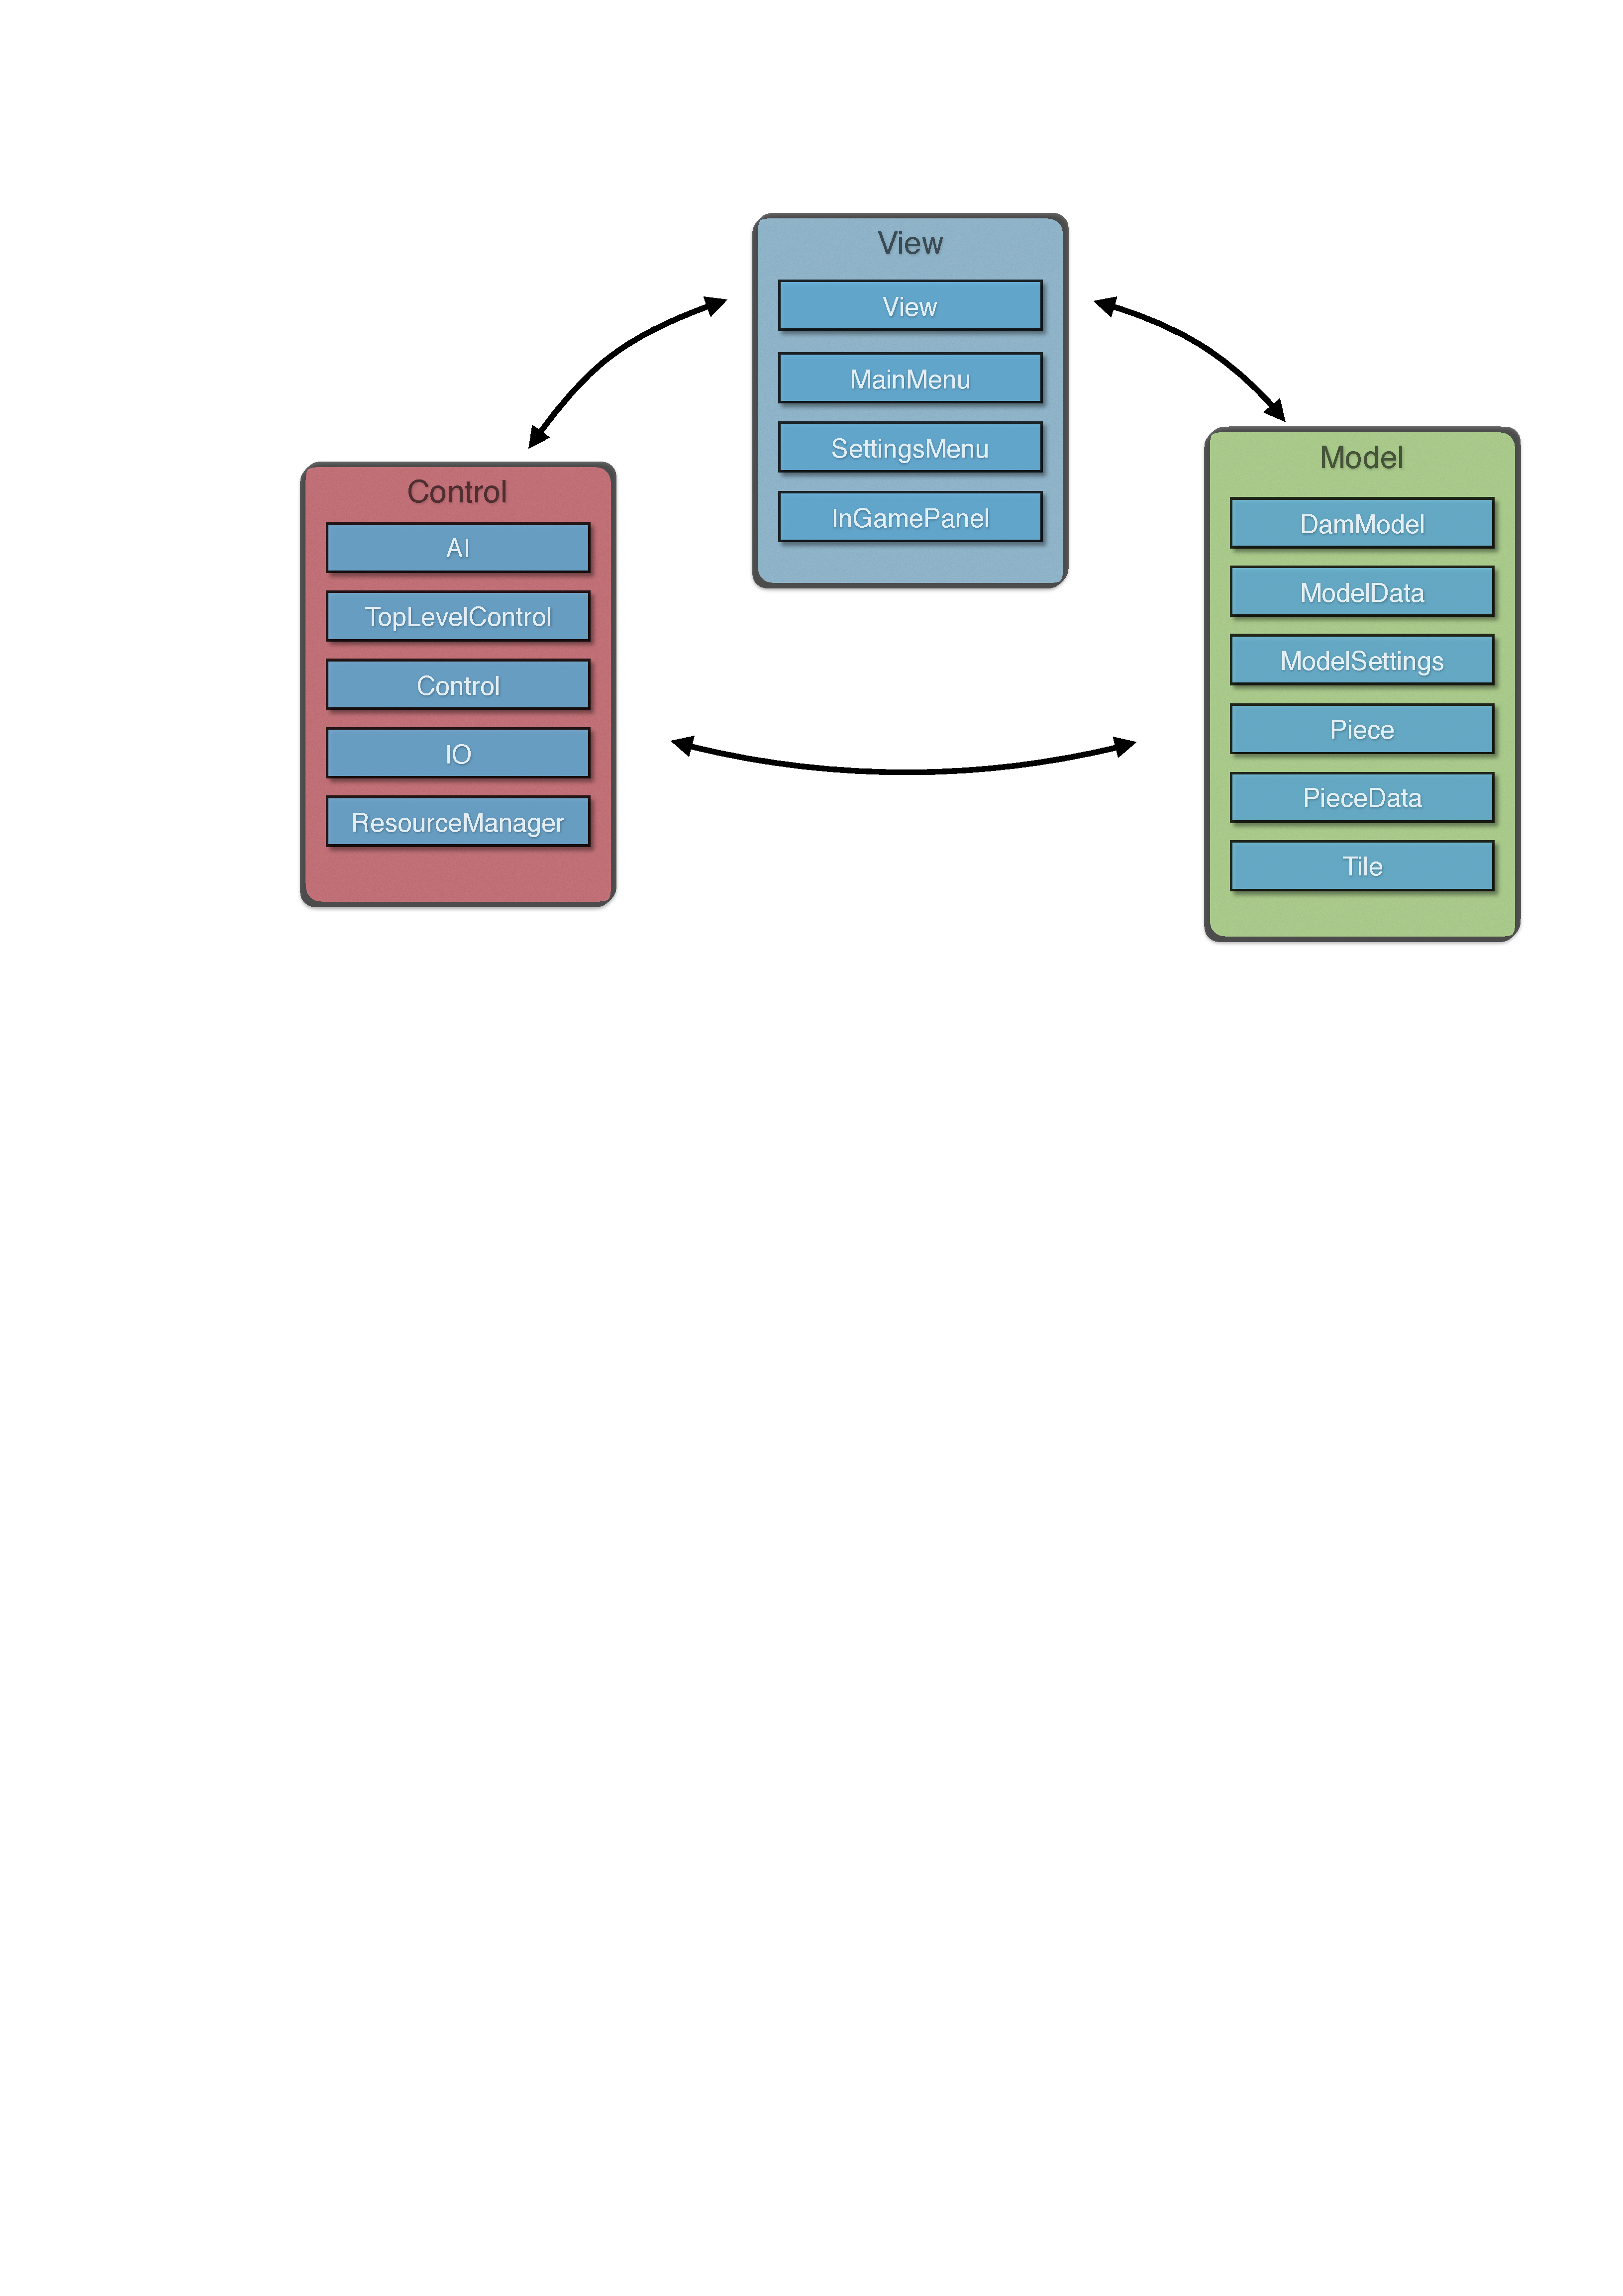
\includegraphics[width = 0.8  \textwidth]{Figurer/Model-View-Control}
\caption{Klasserne der bruges i programmet, delt op efter MVC designmøsntret.}
\label{fig:MVC}
\end{figure}

